\documentclass[a4paper,12pt]{article}
\usepackage[a4paper,top=1.5cm,left=2.1cm,right=2.1cm,bottom=1.8cm,includehead,includefoot]{geometry}
\usepackage[T1]{fontenc}
\usepackage[utf8]{inputenc}
\usepackage[english,bulgarian]{babel}
\usepackage{amssymb,amsmath, oz, mathrsfs}
\usepackage{url}
\usepackage{graphicx}
\usepackage{color,colortbl}
\usepackage{float}

\newtheorem{thm}{Теорема}[section]
\newtheorem{stm}{Твърдение}[section]
\newtheorem{lemma}{Лема}[section]
\newtheorem{defn}{Дефиниция}[section]
\newtheorem{example}{Пример}[section]
\newenvironment{mproof}{\paragraph{Доказателство}}{\hfill$\square$}

\DeclareMathOperator*{\argmax}{arg\,max}
\DeclareMathOperator*{\argmin}{arg\,min}

\makeatletter
\newcommand{\xRightarrow}[2][]{\ext@arrow 0359\Rightarrowfill@{#1}{#2}}
\newcommand{\dslash}{\slash\slash}
\makeatother

\begin{document}
\thispagestyle{empty}
\noindent\begin{minipage}{0.3\textwidth}

\includegraphics[width=10mm,scale=0.5]{figures/logo.jpg}
\end{minipage}%
\hfill%
\begin{minipage}{0.6\textwidth}\raggedleft
Катедра Математическа логика и приложения\\
Факултет по Математика и Информатика\\
Софийски Университет\\
\end{minipage}
\noindent\makebox[\linewidth]{\rule{\textwidth}{1pt}} 
\begin{center}
\begin{minipage}{0.75\linewidth}
    \centering
    \vspace{3cm}
    {\Large \textbf{Заглавие на дипломната работа на много редове}}\par
    \vspace{3cm}
    Дипломна работа\\ на\\ Нели Велиславова Хатева\\ студент специалност Информатика\\ ФН М29245\par
    \vspace{3cm}
    Ръководител \\доц. д-р Стоян Михов\par
    \vspace{3cm}
    2020 \par
    \vspace{3cm}
\end{minipage}
\end{center}
\clearpage

\tableofcontents
\listoffigures
\listoftables
\clearpage

\section{Увод}

  $\hspace*{1mm}$ В компютърните науки компресирането представлява кодиране на данни с цел намаляване на обема им.
  Данните могат да представляват както звуци и изображения, така и текст. Компресирането може да бъде с или без загуба на информация.
  При компресиране без загуба на информация оригиналните данни могат да бъдат възстановени изцяло, докато
  при компресиране със загуба на информация декомпресираните данни се отличават от оригиналните.
  Възниква и въпросът за компресиране на речник от думи на даден естествен език.

  $\hspace*{1mm}$ Всеки речник от думи на даден естествен език е краен списък, който може да се представи с математическия апарат на крайните автомати.
  Това представяне е широко използвано заради компактността му и множеството алгоритми за работа с него. Въпреки това, в много статии
  \cite{citation01, citation02, citation03, citation04} се разглеждат различни формализми, които компресират паметта за това представяне.
  Общото при тези подходи е, че езикът на изходния автомат не се променя, тоест компресирането е без загуба на информация.
  Фокусът на тази дипломна работа е компресията на естествен език със загуба на информация, като се изследва зависимостта между размера на паметта и различията в оригиналния
  и новополучения език.
  
\pagebreak

\section{Мотиви и интуиция}
  $\hspace*{1mm}$ Естествените езици подлежат на различни класификации спрямо набор от различни критерии. Една възможна класификация на езиците е морфологичната и
  типологичната класификация. Тя представлява групиране на езиците въз основа на граматичните отношения. Спрямо тази класификация има четири групи езици:
  инкорпориращи (полисинтетични), изолиращи (коренни), аглутиниращи и флективни. На практика повечето езици проявяват характеристики от различните групи и не могат
  еднозначно да се класифицират, но като цяло всички индоевропейски езици попадат в графата на флективните езици. За тях характерно е, че основното значение
  на думата се носи от нейния корен, а за изразяване на граматичнате категории се използват разнообразни флективни елементи.
  Забелязват се отпределени правила при употребата на флексиите, както и излючения от тези правила.
  Такива изключения възникват поради фонетични особености при произношение на думите, поради исторически причини и ред други.
  За пример в английския език множественото число на повчето думи се образува като към формата за единствено число прибавим \textbf{\emph{s}} на края.
  Но има думи, които са изключение от това правило. Например множественото число на думите,
  завършващи на \textbf{\emph{y}}, предшествано от съгласна, в единствено число, се образува като от основната форма премахнем \textbf{\emph{y}} и
  добавим \textbf{\emph{ies}}. Други пример за изключения при озбразуването на множествено число в английския език са двойките
  \textbf{\emph{foot}} - \textbf{\emph{feet}}, \textbf{\emph{person}} - \textbf{\emph{people}}. Примери в българския език за изключения са думи с така наречените
  променливо \textbf{\emph{я}} (\textbf{\emph{бял}} - \textbf{\emph{бели}}) и подвижно \textbf{\emph{ъ}} (\textbf{\emph{връх}} – \textbf{\emph{върхове}}).
  Универсален пример за изключения от правилото са думи, които имат форма само за единствено число (singulare tantum) или само за множествено число (plurale tantum).
  Примери за плуралия тантум в българския език са думите \textbf{\emph{трици}}, \textbf{\emph{въглища}}, \textbf{\emph{финанси}}, \textbf{\emph{очила}},
  \textbf{\emph{дънки}}, \textbf{\emph{джинси}}, а за сингулария тантум - \textbf{\emph{нефт}}, \textbf{\emph{захар}}, \textbf{\emph{ориз}}, \textbf{\emph{мас}},
  \textbf{\emph{желязо}} \cite{citation05}.

  Такива словоформи водят до увеличаване на размера на автомата, с който представяме езика.
  Ако премахнем словоформите, които са изключения от правилата за спрежение, и ги заменим със словоформи, образувани по правилата,
  тогава паметта за представянето на автомата ще бъде по-малка.
  Това се вижда лесно от следния пример:

\begin{figure}[H]
  \centering
  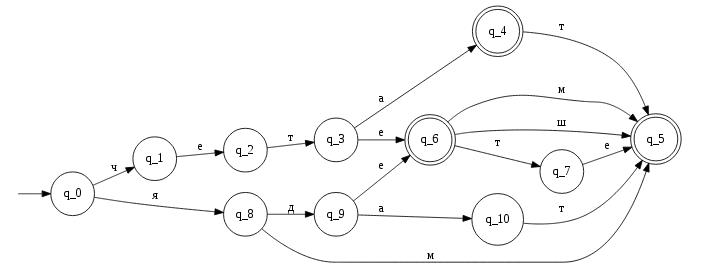
\includegraphics{figures/example1.jpg}
  \caption{Автомат, разпознаващ словоформите \textbf{\emph{ям}}, \textbf{\emph{ядеш}}, \textbf{\emph{яде}},
  \textbf{\emph{ядем}}, \textbf{\emph{ядете}}, \textbf{\emph{ядат}},
  \textbf{\emph{чета}}, \textbf{\emph{четеш}}, \textbf{\emph{чете}},
  \textbf{\emph{четем}}, \textbf{\emph{четете}}, \textbf{\emph{четат}}}
\end{figure}

\begin{figure}[H]
  \centering
  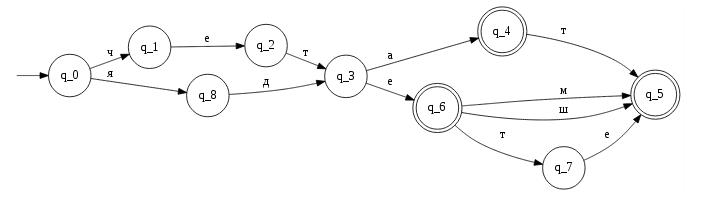
\includegraphics{figures/example2.jpg}
  \caption{Автомат, разпознаващ словоформите \textbf{\emph{яда}}, \textbf{\emph{ядеш}}, \textbf{\emph{яде}},
  \textbf{\emph{ядем}}, \textbf{\emph{ядете}}, \textbf{\emph{ядат}},
  \textbf{\emph{чета}}, \textbf{\emph{четеш}}, \textbf{\emph{чете}},
  \textbf{\emph{четем}}, \textbf{\emph{четете}}, \textbf{\emph{четат}}}
\end{figure}

  Фигура 1. визуализира автомата, който разпознава словоформите
  \textbf{\emph{ям}}, \textbf{\emph{ядеш}}, \textbf{\emph{яде}},
  \textbf{\emph{ядем}}, \textbf{\emph{ядете}}, \textbf{\emph{ядат}},
  \textbf{\emph{чета}}, \textbf{\emph{четеш}}, \textbf{\emph{чете}},
  \textbf{\emph{четем}}, \textbf{\emph{четете}}, \textbf{\emph{четат}}.
  Автоматът се състои от 11 състояния и 16 прехода.
  Фигура 2. визуализира автомата, който разпознава словоформите
  \textbf{\emph{яда}}, \textbf{\emph{ядеш}}, \textbf{\emph{яде}},
  \textbf{\emph{ядем}}, \textbf{\emph{ядете}}, \textbf{\emph{ядат}},
  \textbf{\emph{чета}}, \textbf{\emph{четеш}}, \textbf{\emph{чете}},
  \textbf{\emph{четем}}, \textbf{\emph{четете}}, \textbf{\emph{четат}}.
  Автоматът се състои от 9 състояния и 12 прехода. Този автомат се е получил, като сме премахнали словоформата \textbf{\emph{ям}} и сме я заменили със словоформата
  \textbf{\emph{яда}}. Това води до намаляване на размера на автомата с 2 състояния и 4 прехода.

\pagebreak

\section{Рекурентни невронни мрежи и крайни автомати}

Изкуствените невронни мрежи са математически модели, които представляват композиция на функции с дадени свойства (монотонност, ограниченост). Рекурентните невронни мрежи са частен случай, при който входът на мрежата е крайна редица, като за всеки елемент от редицата прилагаме последователно функция $F$, която зависи от дадения елемент и предходната стойност на функцията. Неформално, при дадена входна редицата $x_1, \ldots, x_T$ пресмятаме редицата от стойностите на функцията $h_0, h_1, \ldots, h_T$, като $h_t = F(h_{(t-1)}, x_t) = \sigma(x_tW_h + h_{(t-1)}U_h + b_h)$. Първият член на редицата $h_0$ обикновенно е отнапред зададен и е константа. Елементите на редицата от стойностите на функцията наричаме скрити състояния, а номера на елементите наричаме момент от времето.

Крайните автомати са друг математически модел, чиито вход е крайна редица, за която прилагаме последователно функция $\Delta$, която зависи от дадения елемент и предходната стойност на функцията, като стойностите, които може да приема функцията са краен брой
$q_t = \Delta(q_{(t-1)}, x_t)$

\section{Общи дефиниции и обозначения}

\begin{defn}
Ако $R \subseteq A_1 \times A_2 \times \ldots \times A_n$ е релация, то с $Proj_iR = \{a_i | (a_1 \ldots a_i \ldots a_n) \in R\}$ означаваме i-тата прокеция на R.
\end{defn}

\begin{defn}
Ако $R$ е релация, с $R^+$ означаваме транзитивното затваряне на $R$.
\end{defn}

\begin{defn}
Азбука $\Sigma$ наричаме всяко крайно множество от символи.
\end{defn}

\begin{defn}
Казваме, че $\alpha$ е дума над азбуката $\Sigma$, ако $\alpha$ е крайна последователност от символи от $\Sigma$ и пишем $\alpha = a_1 a_2 \ldots a_n$, $n \in \mathbb N$.
Дължината на $\alpha$ отбелязваме с $|\alpha|$. Ако $|\alpha| = n$, пишем още $\alpha \in \Sigma^n$.
С $\alpha_1$ отбелязваме $a_1$, с $\alpha_2$ - $a_2$, \ldots, с $\alpha_n$ - $a_n$.
\end{defn}

\begin{defn}
Ако $n, m \in \mathbb N$, $\alpha = a_1 a_2 \ldots a_n \in \Sigma^n$, $\beta = b_1 b_2 \ldots b_m \in \Sigma^m$, тогава думата
$\alpha . \beta = a_1 a_2 \ldots a_n . b_1 b_2 \ldots b_m = a_1 a_2 \ldots a_n b_1 b_2 \ldots b_m \in \Sigma^{n+m}$ наричаме конкатенация на думите $\alpha$ и $\beta$.
\end{defn}

\begin{defn}
Със $\varepsilon$ означаваме празната дума (с дължина 0).
\end{defn}

\begin{defn}
Множеството от всички думи над азбука $\Sigma$ бележим със $\Sigma^*$, където $\Sigma^* = \bigcup\limits_{n=0}^{\infty} \Sigma^n$.
\end{defn}

\begin{defn}
Език L над азбука $\Sigma$ наричаме всяко подмножество на $\Sigma^*$.
\end{defn}

\begin{defn}
Краен детерминиран автомат наричаме нареденната петторка $A = ( \Sigma, Q, s, F, \delta )$, където
$\Sigma$ е крайна азбука, Q е крайно множество от състояния, $s \in Q$ е началното състояние, $F \subseteq Q$ е множеството от финални състояния,
$\delta : Q \times \Sigma \pfun Q$ е частична функция на преходите.
\end{defn}

\begin{defn}
Път в крайния детерминиран автомат $A = ( \Sigma, Q, s, F, \delta )$ наричаме последователността от преходи
$((q_1, a_1), q_2), ((q_2, a_2), q_3), \ldots, ((q_n, a_n), q_{n+1})$, където за $\forall i \in \{1, 2, \ldots, n\} \;\delta(q_i, a_i)=q_{i+1}$.
Такъв път означаваме с $\pi: q_1 \xrightarrow{a_1} q_2 \xrightarrow{a_2} q_3 \xrightarrow{a_3} \ldots \xrightarrow{a_{n  - 1}} q_n \xrightarrow{a_n} q_{n+1}$.
$q_1$ наричаме начало на $\pi$, $q_{n + 1}$ - край на $\pi$, $a_1 a_2 \ldots a_n$ - етикет на $\pi$, n - дължина на $\pi$.
\end{defn}

\begin{defn}
Крайният детерминиран автомат $A = ( \Sigma, Q, s, F, \delta )$ наричаме ацикличен, ако всеки път в А
$\pi: q_1 \xrightarrow{a_1} q_2 \xrightarrow{a_2} q_3 \xrightarrow{a_3} \ldots \xrightarrow{a_{n  - 1}} q_n \xrightarrow{a_n} q_{n+1}$
е такъв, че за $\forall i \in \{1, 2, \ldots, n+1\}$ $\forall j \in \{1, 2, \ldots, n+1\}$ $i \neq j$ $\implies$ $q_i \neq q_j$.
\end{defn}

\begin{defn}
Рефлексивното и транзитивно затваряне на $\delta$ е частичната функция $\delta^* : Q \times \Sigma^* \pfun Q $, която се дефинира по следния начин:
\begin{enumerate}
 \item[1)] $\delta^*(q, \varepsilon) = q$
 \item[2)] $\delta^*(q, a_1 a_2 \ldots a_n) = \delta^*(\delta(q, a_1), a_2 \ldots a_n)$
\end{enumerate}
\end{defn}

\begin{stm}
Нека $A = (\Sigma, Q, s, F, \delta)$ е краен детерминиран автомат. \\$\delta^*(q_1, w) = q_n$ $\Leftrightarrow$ съществува път
$\pi: q_1 \xrightarrow{w_1} q_2 \xrightarrow{w_2} q_3 \xrightarrow{w_3} \ldots \xrightarrow{w_{|w| - 1}} q_{n - 1} \xrightarrow{w_{|w|}} q_n$.
\end{stm}

\begin{defn}
Нека $A = (\Sigma, Q, s, F, \delta)$ е краен детерминиран автомат и $q \in Q$. Тогава $\delta_q = \left.{\delta}\right|_{\{q\} \times \Sigma}$.
\end{defn}

\begin{defn}
Нека $A = (\Sigma, Q, s, F, \delta)$ е краен детерминиран автомат и $q \in Q$. Тогава множеството
$\vec{L}_A(q) = \{w \in \Sigma^* | \delta^*(q, w) \in F\}$ наричаме десен език на състоянието q в автомата A.
\end{defn}

\begin{defn}
Нека $A = (\Sigma, Q, s, F, \delta)$ е краен детерминиран автомат. Език на автомата А наричаме множеството
$L(A) = \vec{L}_A(s)$.
\end{defn}

\begin{defn}
Нека $A = (\Sigma, Q, s, F, \delta)$ е краен детерминиран автомат. Казваме, че състоянията $q_1$ и $q_2$ $\in Q$ са еквивалентни,
ако $\vec{L}_A(q_1) = \vec{L}_A(q_2)$.
\end{defn}

\begin{defn}
Нека $A = (\Sigma, Q_A, s_A, F_A, \delta_A)$ е краен детерминиран автомат. Казваме, че А е минимален, ако за всички
крайни детерминирани автомати $B = (\Sigma, Q_B, s_B, F_B, \delta_B)$, такива че L(A) = L(B), $|Q_A|\;\leq\;|Q_B|$.
\end{defn}

\begin{thm}
Минималният автомат A за даден език L е единствен с точност до изоморфизъм.
\end{thm}

\begin{defn}
Нека $A = (\Sigma, Q_A, s_A, F_A, \delta_A)$ е краен детерминиран автомат и $q \in Q_A$ е произволно състояние. $q$ наричаме достижимо, ако
$\exists w_1 \in \Sigma^* \; \delta_A(s_A, w_1) = q$.
\end{defn}

\begin{defn}
Нека $A = (\Sigma, Q_A, s_A, F_A, \delta_A)$ е краен детерминиран автомат и $q \in Q_A$ е произволно състояние. $q$ наричаме кодостижимо, ако
$\exists w_2 \in \Sigma^* \; \delta_A(q, w_2) \in F_A$.
\end{defn}

\begin{defn}
Нека $A = (\Sigma, Q_A, s_A, F_A, \delta_A)$ и $B = (\Sigma, Q_B, s_A, F_B, \delta_B)$ са крайни детерминирани
автомати. B = trim(A), ако $Q_B = \{q | q \in Q_A \;\&\; \exists w_1 \in \Sigma^* \; \delta_A(s_A, w_1) = q \;\&\; \exists w_2 \in \Sigma^* \; \delta_A(q, w_2) \in F_A\} $,
$\delta_B = \left.{\delta_A}\right|_{Q_B \times \Sigma}$ и $F_B = F_A \cap Q_B$.
\end{defn}

\begin{defn}
С $\mathbb{R}$ бележим множеството на реалните числа.
\end{defn}

\begin{defn}
С $\mathbb{N}$ бележим множеството на естествените числа.
\end{defn}

\begin{defn}
С $\mathbb{M}_{m \times n} (\mathbb{R})$ бележим пространството на матриците с размер ${m \times n}$ и с елементи от множеството на реалните числа $\mathbb{R}$.
\end{defn}

\begin{defn}
Ако $A \in \mathbb{M}_{m \times n} (\mathbb{R})$ е матрица, то елементите на $A$ бележим с $a_{i,j}$, където $i$ е номерът на реда, а $j$ - номерът на стълба. \\
$A = \begin{bmatrix}
  a_{0,0}     & a_{0,1}     & \dots  & a_{0,(n-1)} \\ 
  a_{1,0}     & a_{1,1}     & \dots  & a_{1,(n-1)} \\ 
  \vdots      & \vdots      & \ddots & \vdots \\
  a_{(m-1),0} & a_{(m-1),1} & \dots  & a_{(m-1),(n-1)} \\ 
\end{bmatrix}$
\end{defn}

\begin{defn}
Ако $A \in \mathbb{M}_{m \times n} (\mathbb{R})$ с $A_{i, *}$ бележим $i$-тия ред на матрицата.
\end{defn}

\begin{defn}
Ако $A \in \mathbb{M}_{m \times n} (\mathbb{R})$ с $A_{*, j}$ бележим $j$-тия стълб на матрицата.
\end{defn}

\begin{defn}
С $I_n$ бележим единичната матрица $\begin{bmatrix}
  1      & 0      & \dots  & 0 \\ 
  0      & 1      & \dots  & 0 \\ 
  \vdots & \vdots & \ddots & \vdots \\
  0      & 0      & \dots  & 1 \\ 
\end{bmatrix}$ $\in \mathbb{M}_{n \times n} (\mathbb{R})$ .
\end{defn}

\begin{defn}
С $O_{n,m}$ бележим нулевата матрица $\begin{bmatrix}
  0      & 0      & \dots  & 0 \\ 
  0      & 0      & \dots  & 0 \\ 
  \vdots & \vdots & \ddots & \vdots \\
  0      & 0      & \dots  & 0 \\ 
\end{bmatrix}$ $\in \mathbb{M}_{n \times m} (\mathbb{R})$ .
\end{defn}

\begin{defn}
С $\mathcal{U}(a,b)$ бележим равномерното разпределение.
\end{defn}

\begin{defn}
С $\mathcal{N}(\mu, \sigma^2)$ бележим нормалното разпределение.
\end{defn}

\begin{defn}
$\tanh(x) = \frac{e^x - e^{-x}}{e^x + e^{-x}}$
\end{defn}

\begin{defn} $ReLU(x)= max(0, x)$
\end{defn}

\pagebreak

\section{Формална постановка на задачата}

Даден е краен език $L = \{\alpha_1, \alpha_2, \ldots, \alpha_{|L|}\}$ над азбука $\Sigma = \{a_1, a_2, \ldots, a_{|\Sigma|}\}$, представляващ естествен език - всички думи в речника и техните словоформи. Тъй като езикът е краен, следователно е регулярен и за него може да построим краен детерминиран ацикличен минимален автомат $A$ с език $L(A) = L$.

\subsection{Модел}

Разглеждаме невронна мрежа, която се сътои от три слоя - слой на влагане, рекурентен слой и  линеен слой. За даден вход - дума $\beta = b_1 b_2 \ldots b_n$ над азбуката $\Sigma$,  връща $y = \begin{bmatrix}
  y_1 \\ 
  1 - y_1 \\ 
\end{bmatrix} \in \mathbb{M}_{2 \times 1} (\mathbb{R})$ . $y_1$ е вероятноста думата $\beta$ да принаджели на $L$. $1 - y_1$ съответно е вероятноста думата $\beta$ да не принаджели на $L$. Невронната мрежа след трениране се използва като бинарен класификатор, който опраделя дали дадена дума $\beta$ принадлежи на $L$ или не спрямо това, коя от двете вероятности $y_1$ и $1 - y_1$ е по-голяма.

\subsubsection{Слой на влагане}

$E \in \mathbb{M}_{e \times |\Sigma|} (\mathbb{R})$ е матрица на влагане, $e \in \mathbb{N}$ е размерът на влагането и е хиперпараметър на мрежата. 
На всяка буква от азбуката $a_i$ съпоставяме $E_{*, i} \in \mathbb{M}_{e \times 1} (\mathbb{R})$. Елементите на матрицата $E$ наричаме тегла на слоя на влагане и инизиализираме от $\mathcal{N}(0, 1)$ или с единичната матрица $I_e$ при $e =\:|\Sigma|$ . Техният брой е $e\:\cdot |\Sigma|$. След тази стъпка получаваме редицата $E_{*, i_1}E_{*, i_2} \ldots E_{*, i_n} = x_1 x_2 \ldots x_n$, където $\forall i \in \{1, \ldots, n\} \: x_i \in \mathbb{M}_{e \times 1} (\mathbb{R})$

\subsubsection{Рекурентен слой}

За всеки момент от времето $t \in \{1, 2, \ldots, n\}$ дефинираме скритото състояние $h_t \in \mathbb{M}_{d \times 1} (\mathbb{R})$ като

\begin{equation} \label{eq:1}
h_t = \sigma(W_{ih} x_{(t-1)} + b_{ih} + W_{hh} h_{(t-1)} + b_{hh})
\end{equation}

или 

\begin{equation} \label{eq:2}
h_t = \sigma(W_{ih} x_{(t-1)} + W_{hh} h_{(t-1)})
\end{equation}

където:

\begin{itemize}
\item $W_{ih} \in \mathbb{M}_{d \times e} (\mathbb{R})$; $b_{ih} \in \mathbb{M}_{d \times 1} (\mathbb{R})$; $W_{hh} \in \mathbb{M}_{d \times d} (\mathbb{R})$; $b_{hh} \in \mathbb{M}_{d \times 1} (\mathbb{R})$ - тегла на рекурентния слой. Всички се инициализират от $\mathcal{U}(-\sqrt{\frac{1}{d}}, \sqrt{\frac{1}{d}})$. Техният брой е $d^2 + ed + 2d$, ако използваме уравнение (\ref{eq:1}), или $d^2 + ed$, ако използваме уравнение (\ref{eq:2}).
\item $d \in \mathbb{N}$ е размерът на скритото състояние и е хиперпараметър на мрежата
\item $h_0 = O_{d, 1} \in \mathbb{M}_{d \times 1} (\mathbb{R})$ е скритото състояние в момент 0
\item $\sigma$ - $\tanh$ или ReLU
\end{itemize}

Моделът е предложен в \cite{citation06}. Фиксираме $k \in \mathbb{N}$ на брой състояния $\{s_1, s_2, \ldots, s_k\}$, всяко от които е вектор с размер $d \in \mathbb{N}$. Идеята е във всеки момент от време $t$ да имаме вероятност за преход от $h_t$ към състояние измежду фиксираните $k$ на брой. 

За всеки момент от времето $t \in \{1, 2, \ldots, n\}$ дефинираме скритото състояние $h_t' \in \mathbb{M}_{d \times 1} (\mathbb{R})$ като

\begin{equation}
h_t' = {\sum_{i=1}^{k} \alpha_{i} s_i}
\end{equation}

където

\begin{itemize}
 \item $\alpha_{i} = \frac{\exp \left(- \frac{\Vert{h_t - s_i}\Vert}{\tau}\right)}{\displaystyle\sum_{j=1}^{k} \exp \left(- \frac{\Vert{h_t - s_j}\Vert}{\tau}\right)}$ е разстоянието между $h_t$ и $s_i$, нормализирано до разпределение.
 \item $h_t$ получаваме като използваме уравнение (\ref{eq:1}) или уравнение (\ref{eq:2})
 \item $\tau \in \mathbb{R}$ е хиперпараметър на мрежата, който позволява да променяме разпределението. Колкото повече параметърът клони към 0, толкова разпределението се доближава до характеристичната функция за $\{s_1, s_2, \ldots, s_k\}$. Колкото по-голяма е стойността на параметъра, толкова повече разпределението се приближава до равномерното разпределение.
\end{itemize}

\subsubsection{Линеен слой}

\begin{equation} \label{eq:3}
y = A h_n + b
\end{equation}

или

\begin{equation} \label{eq:4}
y = A h_n
\end{equation}

където:

\begin{itemize}
\item $ A \in \mathbb{M}_{2 \times d} (\mathbb{R})$; $b \in \mathbb{M}_{2 \times 1} (\mathbb{R}) $ - тегла на линейния слой. Всички се интициализират от $\mathcal{U}(-\sqrt{\frac{1}{m}}, \sqrt{\frac{1}{m}})$. Техният брой е $2d + 2$, ако използваме уравнение (\ref{eq:3}), или $2d$, ако използваме уравнение (\ref{eq:4}).
\item $y = \begin{bmatrix}
  y_1 \\ 
  y_2 \\ 
\end{bmatrix} \in \mathbb{M}_{2 \times 1} (\mathbb{R})$ - изход от последния слой на невронната мрежа
\end{itemize}

Функцията на невронната мережа е $NN(\beta) = Ah_n + b$.

\subsection{Данни}

За целите на експериментите използваме речника от думи на български език BG Open Office (цитат?). Той се състои от 721 823 думи. Тъй като предложеният модел е класификатор, трябва да разполагаме с множество от думи, които не са в езика (негативни). Тук могат да се изпробват различни подходи за извличане на такива думи от текстове или генерирането им. Избраната стратегия е да генерираме равно по размер множество от негативни думи. За целта разглеждаме 4 операции - замяна на буква на произволна позиция с друга случайна буква от азбуката, вмъкване на произволна буква от азбуката на произволна позиция, изтриване на буква на произволна позиция и размяна местата на две букви на произволна позиция. Докато негативните примери не станат равни на позитивните за всяка дума от езика избираме произволна операция с равна вероятност и я прилагаме върху думата. Ако думата не е вече в множеството на позитивните и негативните примери, я добавяме като негативна дума. (псевдо-код?)

Тъй като тренирането на модела върху всички данни е бавно, избираме подмножество на думите от речника - множеството от думите класифицирани като числителни в българския език (594 думи), които използваме за предварителни експерименти. 

В таблици \ref{table:1} и \ref{table:2} са дадени статистики за дължините на думите в речниците.

\begin{table}[h!]
\centering
\begin{tabular}{|c|c|c|c|}
\hline
& BG Open Office & Негативни \\
\hline
Минимум & 1 & 1\\
\hline
Максимум & 25 & 26\\
\hline
Средно & 10.04 & 10.10\\
\hline
Дисперсия & 5.94 & 6.34\\
\hline
Стандартно отклонение & 2.44 & 2.52\\
\hline
\end{tabular}
\caption{Статистика за дължините на думите в BG Open Office и генерираните негативни думи}
\label{table:1}
\end{table}

\begin{table}[h!]
\centering
\begin{tabular}{|c|c|c|c|}
\hline
& Числителни & Негативни \\
\hline
minimum & 3 & 2\\
\hline
maximum & 18 & 19\\
\hline
средна & 10.47 & 10.48\\
\hline
дисперсия & 9.88 & 10.56\\
\hline
стандартно отклонение & 3.14 & 3.25\\
\hline
\end{tabular}
\caption{Статистика за дължините на думите в BG Open Office, класифицирани като числителни, и генерираните негативни думи}
\label{table:2}
\end{table}

Minimal FSA States: 133 / Finals: 21 / Transitions: 221 (States + Transitions = 354)
Minimal FSA States:  31463 / Finals: 4426 / Transitions: 78338  (States + Transitions = 109801)

Положителните и негативните думи обединяваме в едно множество от примери, което разбиваме по случаен начин на 3 подмножества $TRAIN, DEV, TEST$, където:
\begin{itemize}
 \item $|TRAIN|\:= 0,8|V|$ - множество за трениране
 \item $|DEV|\:= 0,1|V|$ - множество за проверка
 \item $|TEST|\:= 0,1|V|$ - множество за тестване
\end{itemize}

\subsection{Трениране}

Тъй като изхода от невронната мрежа е $y = \begin{bmatrix}
  y_1 \\ 
  y_2 \\ 
\end{bmatrix} \in \mathbb{M}_{2 \times 1} (\mathbb{R})$, за да получим вероятностно разпределение, изолзваме функцията ${Softmax(\vec{x})}_i = \frac{e^{x_i}}{\sum_{j=1}^{K}e^{x_j}}$ . 

Целевата функцията, която искаме да опитимизираме за един пример от тренирочъвните данни е

\begin{equation} \label{eqn}
BinaryCrossEntropyLoss(t, p) = -(t\log(p) + (1-t)\log(1-p))
\end{equation}

където

\begin{itemize}
 \item $t$ е класът на примера от корпуса, в конкретния случай 0 за негативния клас и 1 за позитивния
 \item $p$ - вероятността от модела за позитивния клас
\end{itemize}

(като тренираме на партиди(?), формулата е малко по-различна, тъй като сумираме по всички примери и делим на общия броя в партидата)

MINI-BATCH GRADIENT DESCENT

Целевата функция опитмизараме итеративно с градиентния метод от първи ред Адам, предложен в \cite{citation07}. Имплементацията на $L2$-нормата e предложена в \cite{citation08}. За една итерация или епоха, преди да променим теглата на модела, разглеждаме всички примери от тренировъчното множество. (псевдо код за тренирането? и за Адам, защото в имплементацията се взима от библиотека?)


За оценка на модела ползваме следната формула
\begin{equation} \label{eqn}
Accuracy = \frac{TP + TN}{TP + TN + FP + FN}
\end{equation}

където\\
$TP$ - брой думи, които са в езика и модела е класифицирал като положителни\\
$TN$ - брой думи, които не са в езика и модела е класифицирал като негативни\\
$FP$ - брой думи, които не са в езика, но модела е класифицирал като положителни\\
$FN$ - брой думи, които са в езика, но модела е класифицирал като негативни\\

\subsection{Краен автомат}

От невронната мрежа строим краен детерминиран автомат. В статията \cite{citation06} е предложен подход, при който взимаме думите от тренировъчните данни, прекарваме ги през автомата и броим колко пъти сме минали през даден преход.(псевдо-код?) При този подход полученият автомат ще зависи не само от модела, но и от тренировъчните данни. (въпреки това с него резултатите изглеждат позитивни, тоест получаваме автомат с по-малко състояния и преходи от изходния, да сложа ли резултати и с този подход?)
Друг възможен начин да построим автомата е с обхождане на мрежата в широчина с всички букви от азбуката. Тръгваме от началното състояние и с всички букви от азбуката гледаме в кое от фиксираните състояния стигаме и го добавяме в опашката. (псевдо-код?)

Експериментите сравняват броя състояния и преходи на оригиналния автомат спрямо тези на автомата, получен от невронната мрежа. 

\pagebreak

\section{Експерименти}


Тренираме базовия модел като нагласяме хиперпараметрите на модела ръчно, така че да постигнем оценка на модела над 0.9. Работим със следния модел

\begin{table}[h!]
\centering
\begin{tabular}{|c|c|c|c|c|c|c|c|c|}
\hline
 & TP & TN & FP & FN & Precision & Recall & F1 & Accuracy\\
\hline
TRAIN & 476 & 463 & 8 & 3 & 0.98 & 0.99 & 0.99 & 0.99\\
\hline
DEV & 53 & 56 & 9 & 1 & 0.85 & 0.98 & 0.91 & 0.92\\
\hline
TEST & 59 & 49 & 9 & 2 & 0.87 & 0.97 & 0.91 & 0.91\\
\hline
\end{tabular}
\caption{Оценка на базовия модел за речника от числителни}
\label{table:5}
\end{table}

Хиперпараметри:
- Слой на влагане - теглата не се тренират, а са константа $e =\:|\Sigma|$ 
- Рекурентен слой - $d = 20$ без биас
- линеейн слой - с биас 
Общ брой параметри  922
Най-добра епоха 53

Тъй като броят клъстери е хиперпараметър на алгоритъма за клъстеризация, за определим колко е техният брой провеждаме експеримент, за да видим как зависи оценката на стохастичния модел от броя на състоянията. Ясно е, че ако броят на състоянията е равен на броя уникални вектори оценката ще се запази. Като намаляваме броя на състоянията, очакваме оценката да се влошава. 

\begin{figure}[H]
  \centering
  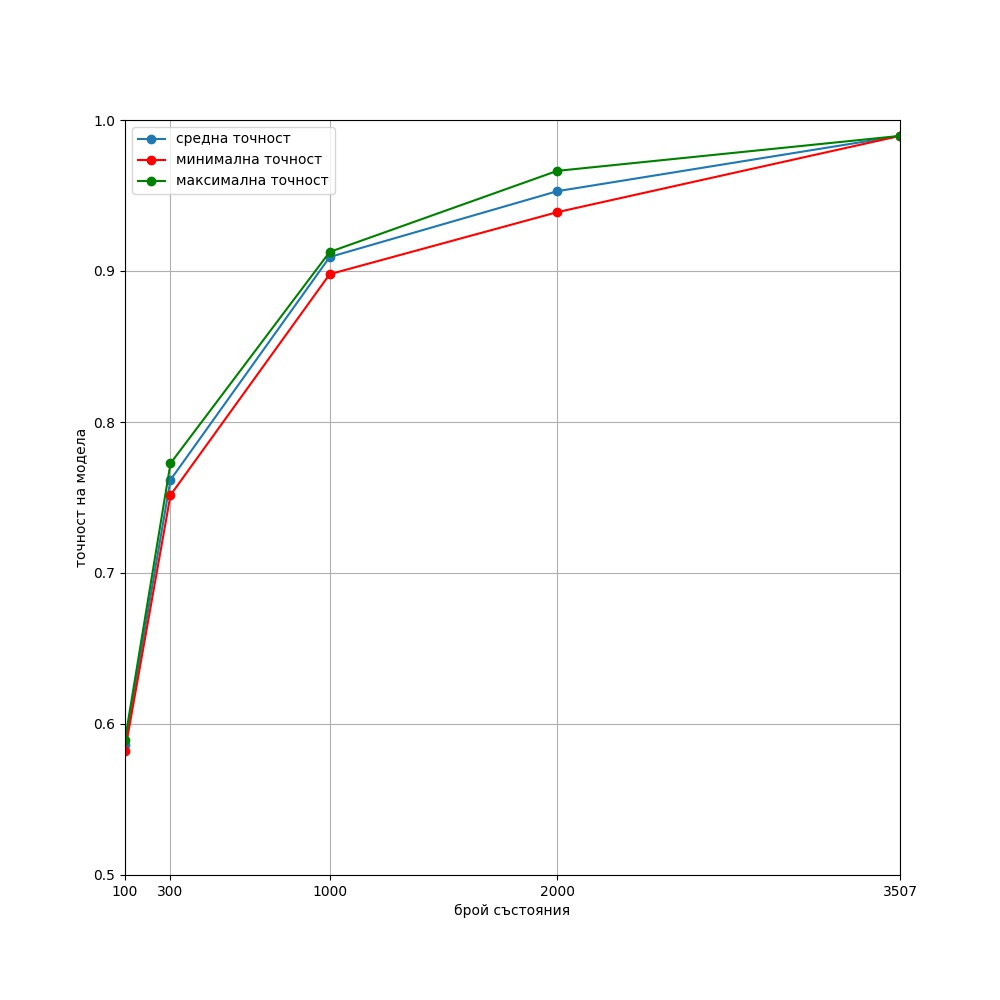
\includegraphics[width=\textwidth,height=\textheight,keepaspectratio]{figures/number-of-states-accuracy.jpg}
  \caption{Изменение на точността на модела спрямо броя състояния}
\end{figure}

\pagebreak

\section{Заключение}

\section{Имплементация}

Приложен е кодът, използван за експериментите. Същият може да бъде намерен и на следния адрес https://github.com/nelly-hateva/rnn2fsa.

TODO

\pagebreak

\begin{thebibliography}{}

\bibitem{citation01}
\newblock Derrick G. Kourie, Bruce W. Watson, Loek Cleophas, and Fritz Venter.
\newblock Failure Deterministic Finite Automata

\bibitem{citation02}
\newblock Henrik Björklund, Johanna Björklund, Niklas Zechner.
\newblock Compression of finite-state automata through failure transitions

\bibitem{citation03}
\newblock Kalin Georgiev.
\newblock Compression of minimal acyclic deterministic FSAs preserving the linear accepting complexity

\bibitem{citation04}
\newblock Jan Daciuk and Jakub Piskorski.
\newblock Gazetteer Compression Technique Based on Substructure Recognition

\bibitem{citation05}
\newblock Руселина Ницолова.
\newblock Българска граматика. Морфология.
\newblock 2008

\bibitem{citation06}
@InProceedings{pmlr-v97-wang19j,  
          title = 	 {State-Regularized Recurrent Neural Networks},  
          author = 	 {Wang, Cheng and Niepert, Mathias},  
          booktitle = 	 {Proceedings of the 36th International Conference on Machine Learning},  
          pages = 	 {6596--6606},  
          year = 	 {2019},  
          editor = 	 {Chaudhuri, Kamalika and Salakhutdinov, Ruslan},  
          volume = 	 {97},  
          series = 	 {Proceedings of Machine Learning Research},  
          address = 	 {Long Beach, California, USA},  
          month = 	 {09--15 Jun},  
          publisher = 	 {PMLR}  
        }

\bibitem{citation07}
@misc{kingma2014adam,
    title={Adam: A Method for Stochastic Optimization},
    author={Diederik P. Kingma and Jimmy Ba},
    year={2014},
    eprint={1412.6980},
    archivePrefix={arXiv},
    primaryClass={cs.LG}
}

\bibitem{citation08} 
@misc{loshchilov2017decoupled,
    title={Decoupled Weight Decay Regularization},
    author={Ilya Loshchilov and Frank Hutter},
    year={2017},
    eprint={1711.05101},
    archivePrefix={arXiv},
    primaryClass={cs.LG}
}

\end{thebibliography}

\pagebreak

\end{document}
